\section{Distributed Execution}
\label{sec:distributed-execution}

Consistency compares independent runs.  A distributed execution places one run
at each participant, and the only change from our framework's
perspective is that participants can learn about inputs at other participants
via messages.  Functional CALM and Complete CALM therefore have a natural
distributed reading.  Sections~\ref{sec:histories}
and~\ref{sec:distributed-consistency} make it precise, including a
convergence guarantee derived from the specification
(Corollary~\ref{cor:convergence}).  We then let systems make their own
commitments, identify coordination with commitment, and state when
conflicting output events cannot be reconciled; Complete CAP then builds on
distributed Complete CALM.

% Subsections 1--2 of the distributed section (input from distributed.tex).

\subsection{Distributed histories}
\label{sec:histories}

A finite set $P$ of \emph{participants} each holds a specification state,
starting at a canonical state $\sigma_S(i_p)$, and changes it only by its own
input and output events.  A participant learns input directly from the
environment or in a message from another participant.  Participants exchange
messages by $\mathsf{send}(m)$ and $\mathsf{receive}(m)$.  A
\emph{message} is a pair $m=(j,d)$ of a cumulative input $j$, or $\varnothing$
if it carries none, and arbitrary other data $d$.  A receive does not change
the specification state; a participant at $(i,R)$ that receives $(j,d)$ with
$j\neq\varnothing$ may incorporate $j$ by its own $\mathsf{input}(k)$ for a
legal common \indesc $k$ of $i$ and $j$, when one exists.

\begin{definition}[Distributed history, consistent cut]
\label{def:distributed-history}
Fix an ordered specification, participants $P$, and an initial input $i_p$
for each.  A \emph{distributed history} $H$ is a finite set of
\emph{history events}, each an occurrence at one participant of an input
event, an output event (Definition~\ref{def:output-event} and
Section~\ref{sec:lifted-output-events}),
$\mathsf{send}(m)$, or $\mathsf{receive}(m)$, with:
\begin{enumerate}
  \item a total local order on each participant's history events;
  \item for each receive, a matching send of the same message at another
        participant, each send matching at most one receive; and
  \item for each participant $p$, its input and output events, in local
        order, form a defined transition sequence from $\sigma_S(i_p)$: each
        is legal at the state where it occurs.
\end{enumerate}
\emph{Happens-before} is the transitive closure of the local orders and of
each send preceding its matching receive.  A \emph{consistent cut} $C$ is a
subset of history events closed under
happens-before~\cite{lamport1978time,chandy1985distributed}; the standard term
is unrelated to our notion of consistency.
\end{definition}

A consistent cut contains a prefix of each participant's history events, so by
item~3
it determines one run per participant.

\begin{definition}[Participant run, endpoint]
\label{def:participant-run}
At a consistent cut $C$, the input and output events of $C$ at participant $p$,
in local order, form its \emph{participant run}, a run
(Definition~\ref{def:run}) whose final state we write $\sigma_p(C)$.  The
\emph{endpoint} of $C$ is $\operatorname{end}(H,C)=(\sigma_p(C))_{p\in P}$.
\end{definition}

\begin{figure}[t]
  \centering
  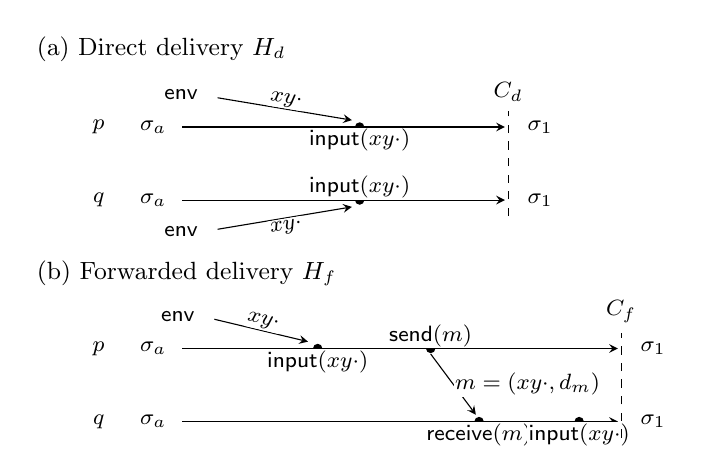
\begin{tikzpicture}[x=.82cm,y=.58cm,>=stealth,
                      every node/.style={font=\footnotesize}]
    % Direct delivery.
    \node[anchor=west,font=\small] at (-1,7.2) {(a) Direct delivery $H_d$};
    \node[anchor=east] at (.35,5.5) {$p$};
    \node[anchor=east] at (.35,3.9) {$q$};
    \node[anchor=west] at (.6,5.5) {$\sigma_a$};
    \node[anchor=west] at (.6,3.9) {$\sigma_a$};
    \draw[->] (1.4,5.5) -- (6.4,5.5);
    \draw[->] (1.4,3.9) -- (6.4,3.9);
    \fill (4.15,5.5) circle (1.7pt);
    \fill (4.15,3.9) circle (1.7pt);
    \node[below,fill=white,inner sep=.5pt] at (4.15,5.5)
      {$\mathsf{input}(xy\cdot)$};
    \node[above,fill=white,inner sep=.5pt] at (4.15,3.9)
      {$\mathsf{input}(xy\cdot)$};
    \node[anchor=east] at (1.8,6.2) {$\mathsf{env}$};
    \node[anchor=east] at (1.8,3.2) {$\mathsf{env}$};
      \draw[->] (1.95,6.14) -- node[midway,above,sloped,fill=white,inner sep=.5pt]
        {$xy\cdot$} (4.03,5.65);
      \draw[->] (1.95,3.26) -- node[midway,below,sloped,fill=white,inner sep=.5pt]
        {$xy\cdot$} (4.03,3.75);
    \draw[dashed] (6.45,3.55) -- (6.45,5.85);
    \node[above] at (6.45,5.85) {$C_d$};
    \node[anchor=west] at (6.6,5.5) {$\sigma_1$};
    \node[anchor=west] at (6.6,3.9) {$\sigma_1$};

    % Forwarded delivery.
    \node[anchor=west,font=\small] at (-1,2.3) {(b) Forwarded delivery $H_f$};
    \node[anchor=east] at (.35,.65) {$p$};
    \node[anchor=east] at (.35,-.95) {$q$};
    \node[anchor=west] at (.6,.65) {$\sigma_a$};
    \node[anchor=west] at (.6,-.95) {$\sigma_a$};
    \draw[->] (1.4,.65) -- (8.15,.65);
    \draw[->] (1.4,-.95) -- (8.15,-.95);
    \node[anchor=east] at (1.75,1.35) {$\mathsf{env}$};
      \draw[->] (1.9,1.29) -- node[midway,above,sloped,fill=white,inner sep=.5pt]
        {$xy\cdot$} (3.35,.8);
    \fill (3.5,.65) circle (1.7pt);
    \node[below,fill=white,inner sep=.5pt] at (3.5,.65)
      {$\mathsf{input}(xy\cdot)$};
    \fill (5.25,.65) circle (1.7pt);
    \node[above,fill=white,inner sep=.5pt] at (5.25,.65)
      {$\mathsf{send}(m)$};
    \fill (6.0,-.95) circle (1.7pt);
    \node[below,fill=white,inner sep=.5pt] at (6.0,-.95)
      {$\mathsf{receive}(m)$};
    \draw[->] (5.25,.53) -- node[midway,right,fill=white,inner sep=.5pt]
      {$m=(xy\cdot,d_m)$} (5.95,-.8);
    \fill (7.55,-.95) circle (1.7pt);
    \node[below,fill=white,inner sep=.5pt] at (7.55,-.95)
      {$\mathsf{input}(xy\cdot)$};
    \draw[dashed] (8.2,-1.3) -- (8.2,1.0);
    \node[above] at (8.2,1.0) {$C_f$};
    \node[anchor=west] at (8.35,.65) {$\sigma_1$};
    \node[anchor=west] at (8.35,-.95) {$\sigma_1$};
  \end{tikzpicture}
  \caption{Two histories from $\sigma_a=\sigma_S(x\cdot\cdot)=(x\cdot\cdot,R_0)$ to
  $\sigma_1=(xy\cdot,R_1)$, with $R_0$ and $R_1$ the tables of
  Figure~\ref{fig:election-frames}(a) and~(b).  In (a) each participant records
  $\mathsf{input}(xy\cdot)$ directly; in (b) $q$ records it after receiving $m$.  Dashed lines are consistent cuts.}
  \label{fig:participant-runs}
\end{figure}

In Figure~\ref{fig:participant-runs}, the input $xy\cdot$ reaches $q$
directly or through a message from $p$.  The histories differ, but at either
cut each participant run is $\mathsf{input}(xy\cdot)$, so both endpoints are
$(\sigma_1,\sigma_1)$.

\subsection{Distributed consistency}
\label{sec:distributed-consistency}

A \emph{continuation} of a history at a consistent cut $C$ is a history $H'$
that extends the history events of $C$ with further history events after
them.  All of $H'$ is a consistent cut of $H'$, its \emph{final cut}.  A
consistent cut $C$ is \emph{confluent at} $j$, for a common \indesc $j$ of
the participants' current inputs, when some continuation at $C$ has a final
cut with endpoint $\bigl((j,R)\bigr)_{p\in P}$ for some $R$: every
participant ends in the same state $(j,R)$.  History events at different
participants are independent, so this holds exactly when the participant runs at $C$ are
confluent at $j$ (Definition~\ref{def:consistency}).

\begin{definition}[Distributed consistency]
\label{def:distributed-consistency}
An ordered specification has \emph{distributed consistency} when, for every
finite participant set, every consistent cut of every history is confluent
at every common \indesc of the participants' current inputs.
\end{definition}

\begin{proposition}[Consistency and distributed consistency]
\label{prop:distributed-consistency}
An ordered specification is consistent if and only if it has distributed
consistency.
\end{proposition}

\begin{proof}[Proof sketch]
The participant runs at a cut are a family of runs, and any family
of runs can be placed at separate participants that exchange no messages.  Full proof in Appendix~\ref{app:proofs-sec4}.
\end{proof}

Both notions are existence claims about transitions
(Section~\ref{sec:scope}).  By Complete CALM,
which reduces to Functional CALM with one output per input, a specification
has distributed consistency exactly when it satisfies Lifted Monotonicity.
For functional specifications,
Corollary~\ref{cor:state-by-input} also gives convergence:

\begin{corollary}[Convergence]
\label{cor:convergence}
In any history of a consistent functional specification, every
participant whose current input at a consistent cut is $j$ is in state
$\sigma_S(j)$.  Participants with the same current input therefore agree,
regardless of message paths, arrival order, or the outputs they emitted.
\end{corollary}

\begin{proof}
Each participant run is a run; apply Corollary~\ref{cor:state-by-input}.
\end{proof}

This is the convergence that strong eventual
consistency~\cite{shapiro2011crdt} asks of replicated state---replicas that
have received the same updates are in equivalent states.  The semilattice merge of CRDTs suffices for it but is not
needed: here it follows directly from any consistent functional specification.  With several outputs per input
this fails even for consistent specifications: in
Figure~\ref{fig:ambiguity-frames}(g), a run that emitted $\{s{\to}\texttt{s1}\}$
has retired the route sets that omit it, while a run at the same input that
emitted nothing keeps them.  Consistency then guarantees that such replicas can
be reconciled, not that they agree.

\paragraph{Message data.}
The data $d$ of a message is any application state other than input that a
participant chooses to send: timestamps, version vectors, non-input-related gossip, votes, etc.  Data
can influence which input and output events occur next at the receiver, but it
never directly changes the receiver's specification state, and nothing in the
definitions above depends on it.  Section~\ref{sec:systems} calls the
rule that makes these choices a participant's \emph{strategy}.  Data can
influence the strategy, but the strategy can decide only within the
specification.
Participants may also share emitted outputs in $d$; this does not change
which cuts are confluent (Appendix~\ref{app:exchanging-outputs}).


\subsection{Systems}
\label{sec:systems}

The histories above use the output events of
Sections~\ref{sec:functional-calm}--\ref{sec:complete-calm}, which apply
exactly the commitments an output requires: they seal the inputs in
$\Sealed_o$ and remove the rows in $\Rejected_o$
(Definition~\ref{def:output-event} and Section~\ref{sec:lifted-output-events}).
Many real systems behave differently.  For example, the registrar of
Section~\ref{sec:election-story} emits $\bot$ and closes the polls in the same
event (Figure~\ref{fig:election-frames}(d)); the output event for $\bot$ does
not require the poll-closing seal, so closing the polls is a design decision of
the system.  Similarly, a lock manager commits to an ordering of ongoing
transactions ($A$ before $B$) without emitting that ordering until later
(Figure~\ref{fig:cc-commitments}(h) below); whether that commitment needs
coordination depends on who else may order the same transactions
(Section~\ref{sec:coordination}).  In this section we show how such
systems can be modeled, by letting them bring bespoke commitments.

\begin{definition}[Commitment]
\label{def:commitment}
A \emph{commitment} is a partial function on
specification states that leaves the current input unchanged and removes a
nonempty set of rows, each with no remaining row at the same input that
\outrel it: whenever $c(i,R)=(i,R')$, we have $R'\subsetneq R$ and
\begin{equation}
  (k,u)\in R\setminus R',\ (k,w)\in R'
  \quad\Longrightarrow\quad
  u\not\OutputOrd w.
  \label{eq:commitment-excludes}
\end{equation}
\end{definition}

The seals and choices of Definition~\ref{def:output-event}
and Section~\ref{sec:lifted-output-events} satisfy this definition: a seal removes
every row at the inputs it seals, and a choice removes the rows in
$\Rejected_o$.  The converse also holds:

\begin{proposition}[Commitments seal inputs or choose outputs]
\label{prop:seal-or-choose}
At each input where a commitment removes rows of the state it is applied to,
it either removes every row there, \emph{sealing} that input, or removes some
outputs and keeps others, \emph{choosing} among them.
\end{proposition}

\begin{proof}
At an input $k$, either no row remains or some does.
\end{proof}

In a functional specification each fiber has one row, so every commitment
seals.  Because each commitment acts on a given state, the classification is
unambiguous.  A seal may remove the last rows that earlier choices left at an
input; attributing the seal across that sequence is a provenance question we do
not pursue.

\begin{definition}[Strategy]
\label{def:strategy}
A \emph{local history} of participant $p$ is a finite sequence of $p$'s history
events, including the messages it
has received.  A \emph{strategy} for $p$ is a nondeterministic transition
function: it maps each local history $\lambda$ of $p$ to a set
$\theta_p(\lambda)$ of output, send, and receive events of $p$, and $p$ next
performs any one of them, or waits.  Input events come from the environment,
not the strategy.
\end{definition}

\begin{definition}[System]
\label{def:system}
A \emph{system} consists of a \emph{commitment basis} $\mathcal B$, the set of
commitments its output events may apply, shared by all participants, and a
strategy $\theta_p$ for each participant $p$ whose output events apply only
commitments from $\mathcal B$.  A distributed history \emph{produced} by the
system consists of environment inputs and events chosen by the participants'
strategies.
\end{definition}

Strategies differ by participant so we can single out replicated
systems, whose participants share one (Appendix~\ref{app:cap-response}); no
result distinguishes participants' commitments, so the basis is shared.

\begin{definition}[Output event of a system]
\label{def:system-output-event}
Let $(i,R)$ be a state and $o\in R(i)$.  An output event $\Out{\gamma}{o}$
under a basis $\mathcal B$ applies a finite, possibly empty sequence
$\gamma=c_1\cdots c_n$ of commitments from $\mathcal B$, each $c_m$ defined at
the state its predecessors leave, leaving a table $R_c$, and then retires rows
and emits $o$, all atomically; $\varepsilon$ is the empty sequence.  The event
is \emph{legal} when $(i,o)\in R_c$ and every row of $R_c$ ruled out by $o$ is
\outrelpast by a retained row that \outrel $o$:
\begin{equation}
  (k,x)\in R_c\setminus R_c[\mathrm{out}\OutputGe o]
  \quad\Longrightarrow\quad
  \exists u\in R_c[\mathrm{out}\OutputGe o](k):\ x\OutputOrd u.
  \label{eq:lifted-validity}
\end{equation}
The event then retires those \outrelpast rows and ends at
$(i,R_c[\mathrm{out}\OutputGe o])$.
\end{definition}

A legal $\Out{\gamma}{o}$ commits at least as much as the $\mathsf{output}(o)$
of Sections~\ref{sec:functional-calm}--\ref{sec:complete-calm}: its commitments
remove the rows in $\Sealed_o$ and $\Rejected_o$
(Lemma~\ref{lem:canonical-commitment-normal-form}), and $\mathsf{output}(o)$ is
the case in which they remove exactly those.  The environment observes $o$, not
$\gamma$.

\paragraph{A transactional example of bespoke commitments.}
The lock manager from the start of this section is one system; multiversion
timestamp ordering (MVTO)~\cite{bernstein1981concurrency} is another, and they
have different bases (Appendix~\ref{app:cc-bases}).  Two-phase locking (2PL)
has $\mathcal B_{\mathrm{2PL}}$, made of ordering commitments
$\mathsf{order}(A,B)$ together with commit, abort, and read commitments; MVTO
has $\mathcal B_{\mathrm{MVTO}}$, made of stamp commitments $\mathsf{stamp}(A)$
together with the same commit, abort, and read commitments.  The ordering
commitments are where they part: $\mathsf{order}(A,B)$ fixes $A$ before $B$ and
nothing else, which no MVTO commitment does, and $\mathsf{stamp}(B)$ places $B$
before every other transaction, which no 2PL commitment does.
Figure~\ref{fig:cc-commitments} shows each at work on a three-transaction
version of the ordering fiber of Figure~\ref{fig:ambiguity-frames}(f).  When
$B$ waits for a lock that $A$ holds, 2PL applies $\mathsf{order}(A,B)$, leaving
$C$'s position open (panel (h)).  When MVTO gives $B$ the first timestamp, it
applies $\mathsf{stamp}(B)$, placing $B$ first (panel (i)).  Both are choices:
they remove serialization orders while the input stays legal, but leave
different alternatives open.  Each is one commitment in the $\gamma$ of an
output event that later emits a full serial order, and neither is the choice
$c_o$ of Section~\ref{sec:lifted-output-events}.

\begin{figure}[t]
  \centering
  \small
  \setlength{\tabcolsep}{5pt}
  \begin{tabular}[t]{@{}l l@{}}
    \multicolumn{2}{@{}l}{(h) 2PL: $A$ locks ahead of $B$}\\
    \toprule
    $\mathrm{in}$ & $\mathrm{out}$ \\ \midrule
    $\{A,B,C\}$ & \sh{$[A,B,C]$} \\
    $\{A,B,C\}$ & \sh{$[A,C,B]$} \\
    $\{A,B,C\}$ & \sh{$[C,A,B]$} \\
    \retired{$\{A,B,C\}$} & \retired{$[B,A,C]$} \\ \strikerow
    \retired{$\{A,B,C\}$} & \retired{$[B,C,A]$} \\ \strikerow
    \retired{$\{A,B,C\}$} & \retired{$[C,B,A]$} \\ \strikerow
    \bottomrule
  \end{tabular}
  \hfill
  \begin{tabular}[t]{@{}l l@{}}
    \multicolumn{2}{@{}l}{(i) MVTO: $B$ receives the first timestamp}\\
    \toprule
    $\mathrm{in}$ & $\mathrm{out}$ \\ \midrule
    $\{A,B,C\}$ & \sh{$[B,A,C]$} \\
    $\{A,B,C\}$ & \sh{$[B,C,A]$} \\
    \retired{$\{A,B,C\}$} & \retired{$[A,B,C]$} \\ \strikerow
    \retired{$\{A,B,C\}$} & \retired{$[A,C,B]$} \\ \strikerow
    \retired{$\{A,B,C\}$} & \retired{$[C,A,B]$} \\ \strikerow
    \retired{$\{A,B,C\}$} & \retired{$[C,B,A]$} \\ \strikerow
    \bottomrule
  \end{tabular}
  \caption{Serial orders of three transactions after one commitment:
  (h) 2PL orders $A$ before $B$; (i) MVTO places $B$ first.  Only complete rows without aborts or reads
  are shown.}
  \label{fig:cc-commitments}
\end{figure}

\paragraph{Canonical runs suffice.}
We call the runs of
Sections~\ref{sec:functional-calm}--\ref{sec:complete-calm} \emph{canonical
runs}, and a \emph{run under a basis} $\mathcal B$ is one whose output events
apply only commitments from $\mathcal B$ (Definition~\ref{def:run-under-basis}).
Although each system can define its own basis, no basis yields behavior that
canonical runs cannot.  Lemma~\ref{lem:canonical-equivalent}
(Appendix~\ref{app:bases}) shows that every run under any basis has an
observably equivalent canonical run: one that accepts the same inputs, emits
the same outputs, and keeps at least the original's rows after each event.  A
system's own commitments can only remove more rows than the canonical ones
would.  In the remainder of the paper we therefore judge consistency on
canonical runs, as in
Sections~\ref{sec:functional-calm}--\ref{sec:complete-calm}.

Consider 2PL on input $\{A,B,C\}$, where $A$ reads a key $x$ that no
transaction writes, and $B$ waits for a lock that $A$ holds on another
key.  2PL's output event reports $A$'s read and applies $\mathsf{order}(A,B)$,
keeping only the rows that can be completed without committing $B$ before $A$.
The canonical run reports the read with no commitment, so it keeps every row reporting the read,
including the one completed by $[B,A,C]$.  When 2PL later emits
$[A,C,B]$, so does the canonical run, and both end with the same table.  The lock committed to $A$ before $B$ earlier than any output
required.

\subsection{Coordination}
\label{sec:coordination}

A commitment is a binding decision that removes behavior the specification
still permits.  What mutexes, locks, timestamps, and agreement protocols have
in common, semantically, is that each implements commitments, by sealing and
choosing (Proposition~\ref{prop:seal-or-choose}).  A commitment needs
coordination, however, only when some other behavior could contradict it:
another run accepting an input it sealed, or emitting an output it chose
against.  We take \emph{coordination} to mean such a commitment, and
\emph{distributed coordination} to mean one that a run at another participant
could contradict.  A
mechanism used without committing is not coordination.  Closing the polls
after every voter has voted still runs the mechanism, but no ballot is left to
seal, so it removes nothing the specification still permits and applies no
commitment.

\begin{definition}[Coordination]
\label{def:coordination}
Let an output event $\Out{\gamma}{o}$
of a run apply a commitment, and let $\mathcal R$ be a set of runs.  The
commitment is \emph{contradicted} in $\mathcal R$ when some run in
$\mathcal R$ accepts an input it seals, or emits, at the same input, an output
it chooses against.  A run or history
\emph{coordinates} relative to $\mathcal R$ when one of its output events
applies a contradicted commitment, and is \emph{coordination-free} relative to
$\mathcal R$ otherwise.  For a specification, $\mathcal R$ is its canonical
runs; for a system, it is the runs it can perform, under any inputs the
environment may supply.  The coordination is \emph{distributed} when the
contradicting run is at another participant of the same history.
\end{definition}

For a specification, every commitment is contradicted: some canonical run
accepts each input that a commitment can seal and emits each permitted
output.  Since any family of canonical runs forms a message-free history
(Proposition~\ref{prop:distributed-consistency}), that run may be at another
participant, so the coordination is also distributed.  For a specification,
then, coordination-free means commitment-free: every output event is some $\Out{\varepsilon}{o}$, which may
still perform output retirements.  This is the sense of
Sections~\ref{sec:functional-calm}--\ref{sec:complete-calm}.

For a system, the answer depends on which runs it can perform, and here seals
and choices differ.  The environment may supply any input to any participant,
so a seal is distributed coordination whenever another participant may receive
the sealed input, whether or not one does in the run at hand.  Closing the
polls before every voter has voted seals the remaining ballots.  It is
coordination in any case, since the environment could deliver a late ballot to
a run that has not yet closed; it is distributed coordination when another
polling station may accept one.  Outputs, by contrast, are chosen only by strategies, so a choice is
contradicted only when some run's strategy may emit the output it rules out.

The next result explains why distributed coordination needs exclusion: a
choice and an output it rules out, at different participants, leave states
that cannot meet at the current input.

\begin{proposition}[Conflicting output events cannot be reconciled]
\label{thm:commitments-require-coordination}
From a state $(i,R)$, let one participant perform an output event after which
no output at $i$ \outrel $x$, and let another perform an output event that
emits $x$.  The two resulting states cannot be brought to a common state with
current input $i$.
\end{proposition}

\begin{proof}[Proof sketch]
After the second event every output at $i$ \outrel $x$, and after
the first none does; since events never add rows, no row at $i$ can be common
to both.  Full proof in Appendix~\ref{app:proofs-sec4}.
\end{proof}

The conflict is confined to the current input.  If $i\InputOrd j$,
$\fiber{i}=\{o,x\}$ with $o$ and $x$ incomparable, and $\fiber{j}=\{u\}$ with
$u$ \outrelpart both, the two states meet once $j$ arrives.  Consistency still
counts this as a failure, since it asks for confluence at the current input
too.  The environment may act on what it observes, through channels the system
does not see, as in Lamport's ``anomalous behavior''~\cite{lamport1978time};
moreover, the input that would reconcile two outputs need not arrive.  Consistency
therefore excludes every observable conflict, including a transient one.

The first event's commitment is a choice against $x$, and it is distributed
coordination exactly when another participant may emit $x$.  The system must
then exclude one of the two events: by a mutex or atomic instruction in shared
memory, by agreement in a distributed system, or by a rule fixed in advance,
such as assigning the choice to a single participant, which keeps the
coordination at that participant and needs no runtime agreement.  Seals are
similar, with input in place of output, but the environment may deliver any
input to any participant, so a seal avoids distributed coordination only if no
other participant can receive the sealed input, a restriction on the
environment that our model does not make.

\paragraph{Locks in a shared-nothing database.}
Consider a database partitioned by key, in which each participant is the lock
manager for its own keys~\cite{stonebraker1986sharednothing}.  Ordering two
transactions on one key is coordination: in another run $B$'s request arrives
first and the owner orders $B$ before $A$.  It is not distributed
coordination, since only the owner orders that key.  It still needs messages,
and a client cut off from the owner cannot get its answer.  A transaction
across keys needs one order, but each owner chooses its part, so the owners'
choices can contradict each other.  Two-phase commit excludes that without
distributed coordination: each owner's prepare is its own commitment, and the
coordinator's decision counts votes from a fixed set of participants, which is
monotone.  Communication and distributed coordination therefore differ.

Confluence is a safety property: some continuation brings the participants to a
common state.  Reaching it is liveness, and a matter of strategy.  Under Lifted
Monotonicity, participants at a common input $j$ can each emit a
$u\in\fiber{j}$ that \outrel everything emitted, without commitment
(Proposition~\ref{prop:exposure-boundary}); choosing $u$ by a shared
deterministic rule terminates once outputs stop.

\subsection{The Complete CAP Theorem}
\label{sec:complete-cap}

Brewer conjectured that a distributed system cannot be consistent, available,
and partition tolerant at once~\cite{brewer2000towards}; Gilbert and Lynch
proved it for a linearizable register~\cite{gilbert2002cap}.  Their theorem
concerns one guarantee, not which guarantees can stay available and
consistent through a partition.  Complete CAP answers that question for any
declared guarantee: a specification of what is correct, together with the
rows whose outputs must stay available.  The answer is that rows emitted apart
must have a common \outnoun wherever their inputs meet; when every permitted
output must stay available, this is Lifted Monotonicity.  A partition does not
change which commitments a specification needs; it removes the ability to make
them jointly, since separated participants cannot agree to seal
an input or make a choice that another could contradict.

\begin{definition}[Partitioned history, Availability, Partition Consistency]
\label{def:partition-notions}
\leavevmode
\begin{enumerate}
  \item \emph{Partitioned history.}  A \emph{partitioned history} divides the
        participants into two or more components and contains no receive whose
        matching send lies in another component; participants still receive
        environment input and emit outputs.
  \item \emph{System.}  Fix a system; we
        require a strategy for each participant of every finite
        participant set and every choice of initial inputs, each depending only
        on its participant's local history.
  \item \emph{Environment.}  The environment is adversarial: it may supply any
        legal input event to any participant.
  \item \emph{Availability.}  A continuation of a partitioned history is
        \emph{local to} a participant $p$ when the system produces it, it
        adds only events of $p$'s component and no input events, and none of
        its receives takes a message sent from another component.  Fix an
        \emph{availability relation} $A\subseteq S$, the rows $(i,o)$ whose
        output $o$ must stay available at input $i$, and write $A(i)$ for its
        fiber $\{o:(i,o)\in A\}$.  The system has \emph{Availability for $A$}
        when, in every partitioned history it produces, each participant $p$,
        ending in state $(i,R)$, can emit each output in $R(i)\cap A(i)$ in
        some continuation local to $p$.  \emph{Availability} is Availability
        for $S$.
  \item \emph{Partition Consistency.}  The system has \emph{Partition
        Consistency} when the final cut of every such history is
        confluent at every common \indesc of the participants' current
        inputs.  The
        continuation that confluence asks for need not stay partitioned and
        need not be produced by the system.
  \item \emph{Consistency on $A$.}  $\Spec$ is \emph{consistent on $A$} when
        every finite set of rows of $A$ with a common \indesc $j$ has a common
        \outnoun in $\fiber{j}$.
\end{enumerate}
\end{definition}

With $A=S$, consistency on $A$ is the common-\indesc condition
(Definition~\ref{def:common-expansion-condition}).  Unlike Availability,
Availability for a smaller $A$ can be met by a system whose output events
commit without coordination, as the remark after Corollary~\ref{cor:complete-cap-S} explains.

\begin{theorem}[Complete CAP]
\label{thm:complete-cap}
For an ordered specification $\Spec$ and an availability relation
$A\subseteq S$, the following are equivalent:
\begin{enumerate}
  \item some system has Availability for $A$ and Partition Consistency;
  \item $\Spec$ is consistent on $A$.
\end{enumerate}
\end{theorem}

\begin{proof}[Proof sketch]
Consider the system whose strategies emit each output of
$A$ by the canonical output event of Section~\ref{sec:complete-calm}.  It has
Availability for $A$, and consistency on $A$ gives the outputs it emits a
common \outnoun wherever their inputs meet.  Conversely, given one
participant per row of $A$, each in its own component, Availability lets each
emit its row's output, and Partition Consistency then supplies the common
\outnoun.  Full proof in Appendix~\ref{app:proofs-sec4}.
\end{proof}

\begin{corollary}
\label{cor:complete-cap-S}
Some system has Availability and Partition Consistency if and only if $\Spec$
satisfies Lifted Monotonicity.  When it does, a commitment-free system has
both: one whose strategies may emit any exposable output $o$ by
$\Out{\varepsilon}{o}$.
\end{corollary}

\begin{proof}[Proof sketch]
With $A=S$, consistency on $A$ is Lifted Monotonicity, and the
exposure boundary makes every
output of the commitment-free system available.  Full proof in Appendix~\ref{app:proofs-sec4}.
\end{proof}

The converse never assumes that the system is commitment-free, so commitments
cannot enlarge the class of specifications that admit a system with
Availability for $A$ and Partition Consistency.  Nor do the commitments of the
canonical system above need coordination.  Under consistency on $A$, the canonical event
for an output of $A$ seals nothing and chooses only against outputs outside
$A$, which the system never emits, so it is
coordination-free (Definition~\ref{def:coordination}).  For $A=S$ it needs no
commitment at all.  For a smaller $A$ such local choices can be necessary: if
$o\in A(i)$ and $x\in\fiber{i}\setminus A(i)$ have no common \outnoun at $i$,
emitting $o$ must choose against $x$.  When consistency on $A$ fails, some
output of $A$ either waits for another component, sacrificing Availability, or
is emitted independently at the cost of Partition Consistency.

\paragraph{Gilbert and Lynch.}
Their theorem is a case of Complete CAP.  Consider a register whose input is the
set of operations a participant knows, with their real-time precedence, and
whose outputs answer every operation of the input as some linearization
does~\cite{herlihy1990linearizability}.  Let $p$'s input be a write of
$v\neq v_0$ and $q$'s a read; the only outputs they permit are the
acknowledgment and $v_0$.  Where the write precedes the read, every output
returns $v$, so $v_0$ has no \outnoun there and $\Spec$ is not consistent on
$S$.  The converse in the proof of Theorem~\ref{thm:complete-cap} needs
Availability only so that $p$ can emit the acknowledgment and $q$ can emit
$v_0$.  Each is the only output its input permits, so it is enough that every
request receive some response, which is Gilbert and Lynch's availability.  It
needs Partition Consistency only to give a common \outnoun of the emitted
outputs, which is what linearizability requires.
Appendix~\ref{app:cap-response} takes precedence from real time, extends
Complete CAP to systems that choose their responses when responses are not
forced, and derives
the theorem in Gilbert and Lynch's asynchronous model.

